\setcounter{section}{72}
\section{Двумерная теорема Минковского. Ее уточнение для замкнутых множеств (б/д). }
\textbf{Двумерная теорема Минковского}. \par

\includegraphics[width=14cm]{images/73_1} \par
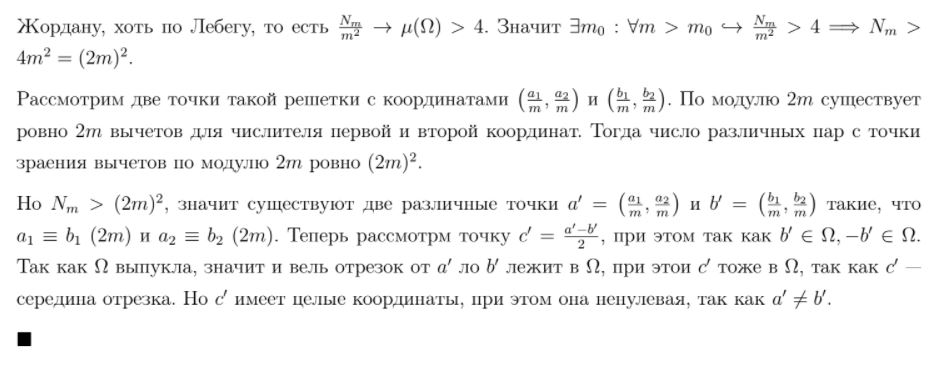
\includegraphics[width=14cm]{images/73_2} \par
\textbf{Уточнение двумерной теоремы Минковского для замкнутых множеств}. \par

\includegraphics[width=14cm]{images/73_3} \par

\section{Применение двумерной теоремы Минковского для передоказательства теоремы Дирихле. Теорема Дирихле о совместном диофантовом приближении (б/д)}
\textbf{Теорема Дирихле}. \par
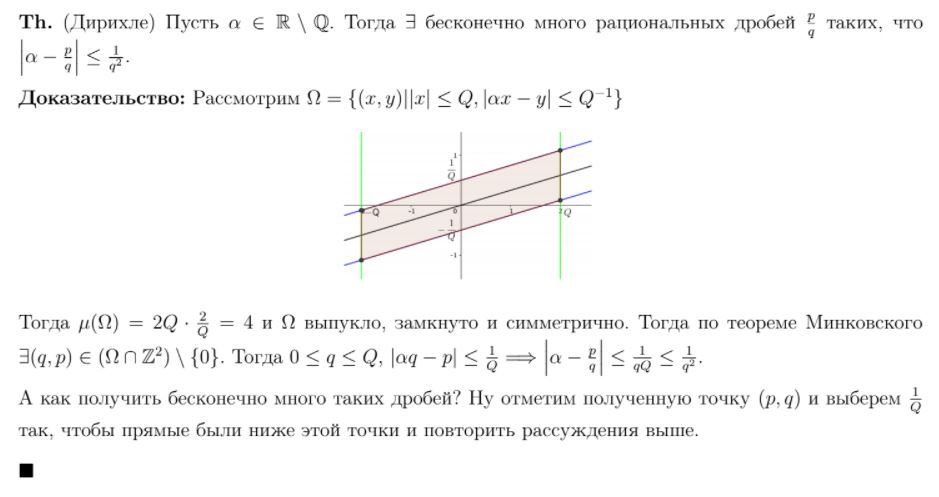
\includegraphics[width=14cm]{images/74} \par
\textbf{Теорема Дирихле о совместном диофантовом приближении}. \par
$\alpha_1, \dots, \alpha_n \notin \mathbb{Q} \Rightarrow \exists$ бесконечно много различных $(p_1/q, \dots, p_n/q): |\alpha_i - p_i/q| \leqslant \frac{1}{q^{1+1/n}}$